Benchmarking-delens fremmeste formål er at finde svar på en række spørgsmål
inden udregningen sættes igang.  Reelt har vi kun en enkelt parameter vi kan
skrue på, nemlig $m$ - antallet af dronninger vi placerer på hver board før vi
genererer et mig job til at regne videre på det board.  Hvilket forhold mellem 

%\subsection{Takaken}
%\subsection{Java port}
%\subsection{Java port v2}
%\subsubsection{Rekursion vs. Iterativ metode}
%\subsubsection{Iterativ med checkpoints}
%\subsection{MiGrid}

\subsection{Lokale tests}

Vi starter med at teste de forskellige udgaver af koden lokalt, så vi har en
baseline at sammenligne med.

Alle lokale tests er kørt på en IBM T43, med en pentium m 1.86Ghz cpu, 

Java koden er kompilet med javac

\begin{verbatim}
alex@roadrunner:~/temp/queens/src/main/java$ javac -version
javac 1.5.0_11
\end{verbatim}

C koden er kompilet med \texttt{gcc -Os -O2 -o nq nqueens.c}

\begin{verbatim}
alex@roadrunner:~/temp/queens/src/main/java$ gcc --version
gcc (GCC) 4.1.2 (Ubuntu 4.1.2-0ubuntu4)
\end{verbatim}

De første tests er kørt på revision 77 (i forbindelse med den iterative test er
udskrivning af debug info til skærmen dog blevet kommenteret ud)

\begin{figure}
\begin{center}
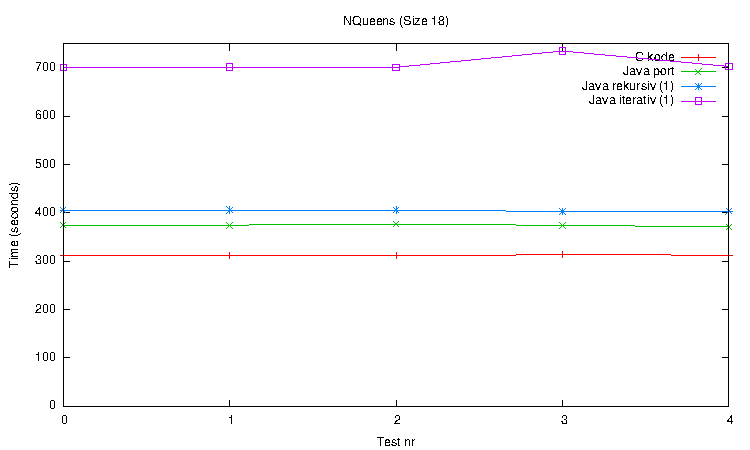
\includegraphics{../benchmarks/b1.pdf}
\caption{insert proper caption here } 
\label{plot:b1}
\end{center}
\end{figure}

Som det ses er C udgaven en smule hurtigere end den direkte java port, der igen
er lidt hurtigere end den paralleliserede udgave af koden, når den kører
rekursivt. Den iterative udgave er væsentlig langsommere..

Den parallelle udgave af koden er i dette tilfælde her kørt med
\texttt{maxSteps} på 1. 

Den næste graf er den rekursive udgave af den parallele kode kørt med forskellig
\texttt{maxSteps}. 

\begin{figure}
\begin{center}
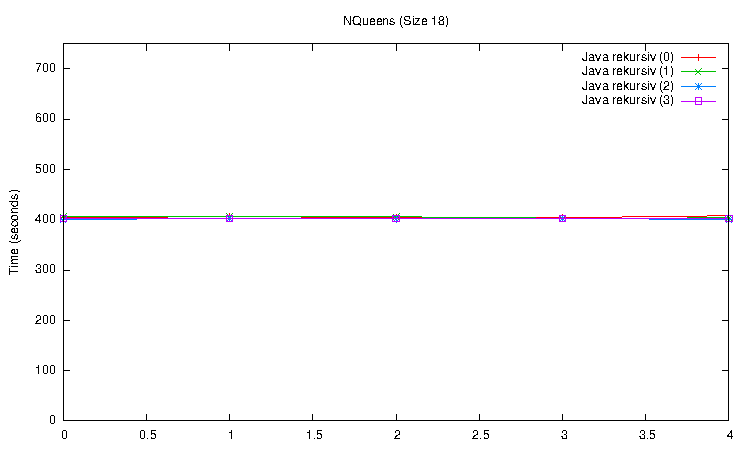
\includegraphics{../benchmarks/b2.pdf}
\caption{insert proper caption here } 
\label{plot:b2}
\end{center}
\end{figure}

Som det ses, har det ikke nogen indflydelse på performance, når det kører
lokalt, der er altså ikke det store overhead ved at generere en masse opgaver og
løse dem bagefter. 

\fixme{hvor mange jobs bliver der lavet for de forskellige maxsteps, indsæt
tabel?}

Alle tests er i første omgang kørt 5 gange, dette blev gjort for at se om
køretiden svingede meget, da dette ikke lader til at være tilfældet vil resten
af testene kun blive kørt 1 gang.. 


Nu skal vi så se på hvor hurtigt det kører når vi smider det efter MiGrid. 
Disse tests er kørt med \texttt{maxSteps} 0 og 1. 


De foregående tests er kørt med kode der bruger \texttt{int} til at gemme resultaterne,
i de næste tests er \texttt{int} skiftet ud med \texttt{BigInteger} (revision
83

Sammenligning af alle benchmarks

\begin{figure}
\begin{center}
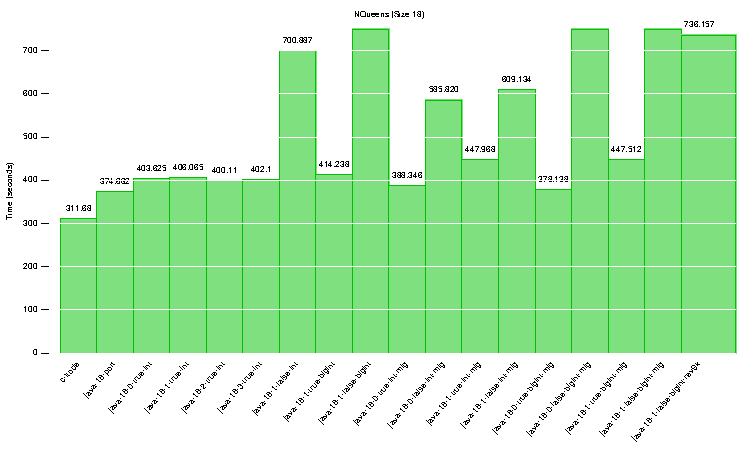
\includegraphics{../benchmarks/b3.pdf}
\caption{insert proper caption here } 
\label{plot:b3}
\end{center}
\end{figure}

\begin{itemize}
\item[1] Takakens C-kode
\item[2] Direkte java port
\item[3] Parallel java port, \texttt{maxSteps}=0, rekursiv, int, lokal
\item[4] Parallel java port, \texttt{maxSteps}=1, rekursiv, int, lokal
\item[5] Parallel java port, \texttt{maxSteps}=2, rekursiv, int, lokal
\item[6] Parallel java port, \texttt{maxSteps}=3, rekursiv, int, lokal
\item[7] Parallel java port, \texttt{maxSteps}=1, iterativ, int, lokal
\item[8] Parallel java port, \texttt{maxSteps}=1, rekursiv, bigint, lokal
\item[9] Parallel java port, \texttt{maxSteps}=1, iterativ, bigint, lokal
\item[10] Parallel java port, \texttt{maxSteps}=0, rekursiv, int, MiG
\item[11], Parallel java port, \texttt{maxSteps}=0, iterativ, int MiG
\item[12], Parallel java port, \texttt{maxSteps}=1, rekursiv, int, MiG
\item[13], Parallel java port, \texttt{maxSteps}=1, iterativ, int, MiG
\item[14], Parallel java port, \texttt{maxSteps}=0, rekursiv, bigint, MiG
\item[15], Parallel java port, \texttt{maxSteps}=0, iterativ, bigint, MiG
\item[16], Parallel java port, \texttt{maxSteps}=1, rekursiv, bigint, MiG
\item[17], Parallel java port, \texttt{maxSteps}=1, iterativ, bigint, MiG
\end{itemize}
